 % LuaLaTeX文書; 文字コーAドはUTF-8
 \documentclass[unicode,12pt, A4j]{ltjsarticle}% 'unicode'が必要
 %\usepackage{luatexja}% 日本語したい
 \usepackage{luatexja-fontspec}
 %\usepackage[hiragino-pron]{luatexja-preset}% IPAexフォントしたい(ipaex)
 \usepackage[hiragino-pron,deluxe,expert,bold]{luatexja-preset}
\usepackage{tikz}
\usetikzlibrary{arrows.meta}
\usetikzlibrary{calc}
 \usepackage[english]{babel}%多言語文書を作成する
 \usepackage{amsmath,amssymb}%標準数式表現を拡大する
 \usepackage{physics}
 \usepackage[subpreambles=true,sort=true]{standalone}
% \renewcommand{\kanjifamilydefault}{\gtdefault}% 既定をゴシック体に
 \usepackage[backend=bibtex,style=phys,articletitle=false,biblabel=brackets,chaptertitle=false,pageranges=false]{biblatex}
 %\usepackage[style=authoryear,backend=bibtex]{biblatex}


 \usepackage{mhchem}
 % あとは欧文の場合と同じ

  \usepackage{caption}
  \usepackage[subrefformat=parens]{subcaption}
\title{東大数学理科後期1996年度}
\author{}
\date{}

\begin{document}
\maketitle

\section{問題1}
$n$を正の整数とし,$n$個のボールを$3$つの箱に分けて入れる問題を考える.ただし,
$1$個のボールも入らない箱があってもよいものとする.以下に述べる$4$つの場合につい
て,それぞれ相異なる入れ方の総数を求めよ.

\begin{enumerate}
\item $1$から$n$まで異なる番号のついた$n$個のボールを,$A$, $B$, $C$と区別された$3$つの
箱に入れる場合,その入れ方は全部で何通りあるか.

\item 互いに区別のつかない$n$個のボールを,$A$, $B$, $C$と区別された$3$つの箱に入れる
場合,その入れ方は全部で何通りあるか.

\item $1$から$n$まで異なる番号のついた$n$個のボールを,区別のつかない$3$つの箱に入
れる場合,その入れ方は全部で何通りあるか.

\item $n$が$6$の倍数$6m$であるとき,$n$個の互いに区別のつかないボールを,区別のつかな
い$3$つの箱に入れる場合,その入れ方は全部で何通りあるか.
\end{enumerate}

\section{問題2}
$3$辺の長さが$BC = 2a$, $CA = 2b$, $AB = 2c$であるような鋭角三角形$\triangle ABC$の
$3$辺$BC$, $CA$, $AB$の中点をそれぞれ$L$, $M$, $N$とする.線分$LM$, $MN$, $NL$に沿っ
て三角形を折り曲げ,四面体をつくる.その際,線分$BL$と$CL$, $CM$と$AM$, $AN$と
$BN$はそれぞれ同一視されて,長さが$a$, $b$, $c$の辺になるものとする.

\begin{enumerate}
\item 線分$MN$, $BL$の中点をそれぞれ$P$, $Q$とする.四面体を組み立てたとき,空間
内の線分$PQ$の長さを求めよ.

\item この四面体の体積を$a$, $b$, $c$を用いて表せ.
\end{enumerate}

\begin{figure}[h]
\centering
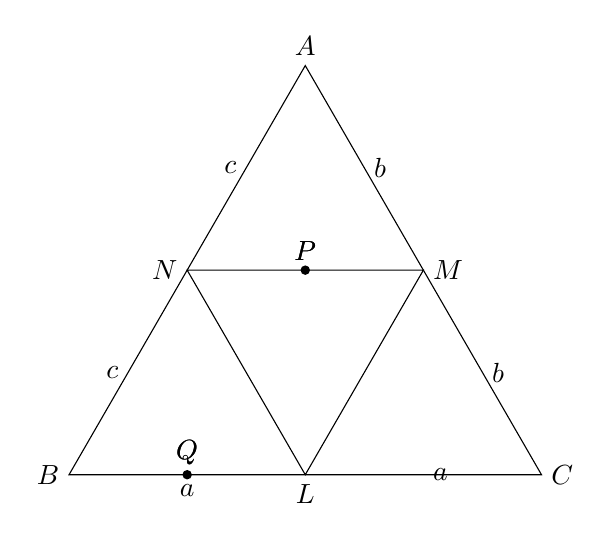
\begin{tikzpicture}[scale=3]
% Triangle vertices
\coordinate (A) at (0,1.732);
\coordinate (B) at (-1,0);
\coordinate (C) at (1,0);

% Midpoints
\coordinate (L) at (0,0);
\coordinate (M) at (0.5,0.866);
\coordinate (N) at (-0.5,0.866);

% P and Q points
\coordinate (P) at (0,0.866);
\coordinate (Q) at (-0.5,0);

% Draw triangle
\draw (A) -- (B) -- (C) -- cycle;

% Draw internal lines
\draw (L) -- (M) -- (N) -- cycle;

% Label vertices
\node[above] at (A) {$A$};
\node[left] at (B) {$B$};
\node[right] at (C) {$C$};
\node[below] at (L) {$L$};
\node[right] at (M) {$M$};
\node[left] at (N) {$N$};
\fill[black] (P) circle (0.02) node[above]{$P$};
\fill[black] (Q) circle (0.02) node[above]{$Q$};
// \node[above] at (P) {$P$};
// \node[above] at (Q) {$Q$};

% Label edges
\node[right] at ($(M)!0.5!(C)$) {$b$};
\node[right] at ($(M)!0.5!(A)$) {$b$};
\node[left] at ($(A)!0.5!(N)$) {$c$};
\node[left] at ($(B)!0.5!(N)$) {$c$};
\node[below] at ($(B)!0.5!(L)$) {$a$};
\node[right] at ($(L)!0.5!(C)$) {$a$};
\end{tikzpicture}
\end{figure}

\section{問題3}
直円柱形の石油タンクが,図のように側面の一母線で水平な地面と接する形に横倒
しになり,地面と接する一点に穴があいて石油が流出しはじめた.倒壊前の石油タンクは
一杯で,$1$時間後の現在までに半分の石油が流出した.単位時間当りの流出量は穴から
測った油面の高さの平方根に比例するという.微分方程式をたてて,このあと何時間何分
で全部の石油が流出するか予測せよ.ただし,分末満は切り捨てよ.

\begin{center}
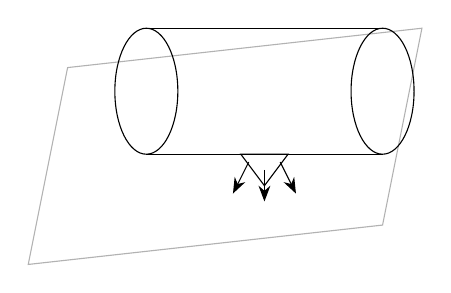
\begin{tikzpicture}

   % 平面(底面)の描画
    \draw[thin,gray!60] (-1.5,-1.5) -- (3,-1) -- (3.5,1.5) -- (-1,1) -- cycle;
    
    % 横向きの円筒を描画
    % 円筒の左側面(円)
    \draw[thin] (0,0.7) ellipse (0.4 and 0.8);
    
    % 円筒の右側面(円)
    \draw[thin] (3,0.7) ellipse (0.4 and 0.8);
    
    % 円筒の上部の線
    \draw[thin] (0,1.5) -- (3,1.5);
    \draw[thin] (0,-0.1) -- (3,-0.1);
    
    % 三角形領域(接地面)
    \draw[thin] (1.2,-0.1) -- (1.5,-0.5) -- (1.8,-0.1) -- cycle;
    
    % 三角形から出る矢印
    \draw[-{Stealth[length=2mm]}] (1.3,-0.2) -- (1.1,-0.6);
    \draw[-{Stealth[length=2mm]}] (1.5,-0.3) -- (1.5,-0.7);
    \draw[-{Stealth[length=2mm]}] (1.7,-0.2) -- (1.9,-0.6);
 

\end{tikzpicture}
\end{center}
\end{document}